% ============================================================================
% Meta-control helps a little, memory decides — full working draft v1
% Built from: docs/research-notes/0008 (skeleton), 0005/0006/0007 (results),
% 0010 (related-work map). Bib: references.bib (copy of docs/references/).
% Venue-agnostic preamble; swap for the venue class (e.g. CoLLAs/PMLR) at submission.
% Build: pdflatex main && bibtex main && pdflatex main && pdflatex main
% ============================================================================
\documentclass[11pt]{article}

\usepackage[margin=1in]{geometry}
\usepackage[T1]{fontenc}
\usepackage[utf8]{inputenc}
\usepackage{amsmath,amssymb}
\usepackage{booktabs}
\usepackage{graphicx}
\usepackage{microtype}
\usepackage[numbers,sort&compress]{natbib}
\usepackage[colorlinks=true,linkcolor=blue!60!black,citecolor=blue!60!black,urlcolor=blue!60!black]{hyperref}
\usepackage{xcolor}

\newcommand{\todo}[1]{\textcolor{red!70!black}{[TODO: #1]}}
\newcommand{\composite}{\textsc{composite}}
\newcommand{\hit80}{\textsc{hit80}}

\title{Meta-Control Helps a Little, Memory Decides:\\
Locating the Catastrophic-Forgetting Bottleneck with a Control Ladder}

\author{Elijah Tabachnik\\
\todo{affiliation / email}}

\date{Draft v1 --- July 2026}

\begin{document}
\maketitle

\begin{abstract}
Neuromodulatory meta-control---an outer policy that sets an inner learner's
plasticity and stability hyperparameters online---is an appealing route to
mitigating catastrophic forgetting in non-stationary reinforcement learning.
We build a controlled instrument for this idea (an outer PPO ``Brain''
controlling a Dyna-style PPO continual learner on a fast-switching MiniGrid
regime schedule) and run the full ladder of controls that reported gains in
this space usually omit: a no-controller tuned-static bottom rung, oracle-timed
and oracle-informed upper bounds on the modulation pathway, and a
zero-forgetting restore ceiling. Three results emerge. \textbf{(1)~A trained
controller helps, and the effect replicates across training seeds:} pooled over
four independently trained Brains, each contrasted against its own frozen
random initialization under a single-variable matched protocol, trained
meta-control improves post-switch recovery by $+0.046$ composite
($p=1.3\times10^{-6}$, $n{=}16$ evaluation seeds per arm; 3 of 4 Brains
individually positive), an estimate that \emph{converges} rather than decays as
evaluation samples grow. \textbf{(2)~The modulation pathway is inert and the
targeted pathology is absent:} feeding ground-truth regime identity through the
learned gating channel does nothing; perfectly timed critic damping
\emph{hurts}; and the dormant-unit fraction falls rather than accumulates over
the run. \textbf{(3)~The bottleneck is knowledge restoration, not learning
dynamics:} a zero-forgetting oracle that restores the learner's stored state at
each regime switch gains $+0.249$ composite on the same instrument---roughly
$5\times$ the trained-controller effect. Along the way, three
small-sample effects that passed initial screens died under replication; we
describe the convergence-vs-decay criterion and protocol-matching discipline
that separated them from the one effect that survived. We argue that the next
lever for task-free continual RL is explicit memory---learning \emph{when} to
snapshot and restore---rather than better hyperparameter meta-control.
\end{abstract}

\section{Introduction}
\label{sec:intro}

Catastrophic forgetting is the tendency of neural learners to overwrite
previously acquired competence when the training distribution shifts. In
reinforcement learning the problem is acute: a policy that alternates between
task regimes pays a relearning cost at every return visit. One family of
remedies is \emph{meta-control}: wrap the learner in an outer controller that
observes training signals and adjusts the learner's hyperparameters online ---
learning rates, exploration and intrinsic-motivation coefficients, replay
behavior, and, in neuromodulation-inspired variants, a learned gating signal
over the network's features. The hypothesis is that the right \emph{schedule}
of plasticity can protect old knowledge and accelerate recovery.

Reported successes of online hyperparameter control in RL are substantial ---
meta-gradients~\citep{xu2018metagradient}, self-tuning
actor-critics~\citep{zahavy2020stac}, population-based
training~\citep{jaderberg2017pbt}, and bandit meta-controllers~\citep{badia2020agent57}
all report large gains --- but, as far as we are aware, all of them are
demonstrated on \emph{stationary} single-task problems, and none is compared
against the control that matters for the continual setting: the same learner
with well-tuned \emph{static} hyperparameters, measured on recovery after
distribution shifts. Meanwhile, the AutoRL literature flags
dynamic-versus-static configuration as an open problem~\citep{parkerholder2022autorl},
and careful tuning studies show static configurations are stronger baselines
than commonly assumed~\citep{eimer2023hyperparameters,andrychowicz2021whatmatters}.

This paper asks the control-ladder question directly. We build a two-level
instrument --- an outer PPO ``Brain'' that observes 19 aggregate training
signals and controls 7 scalar hyperparameters plus an 8-dimensional
neuromodulatory gating code of a Dyna-style PPO continual
learner~\citep{schulman2017ppo,sutton1990dyna} --- and we measure every rung of
the ladder on a frozen benchmark with a frozen scorer: no controller at all,
an untrained controller, the trained controller, oracle-assisted versions of
the controller's individual pathways, and a zero-forgetting oracle that upper
bounds what \emph{any} intervention could achieve by restoring the learner's
own stored state at each switch.

\paragraph{Contributions.}
\begin{enumerate}
  \item \textbf{A positive, controlled, replicated result for trained
  hyperparameter meta-control} (\S\ref{sec:replication}): across four
  independently trained Brains, each evaluated against its own frozen random
  initialization under a single-variable matched protocol, training the
  controller is worth $+0.046$ composite ($\approx$9\% relative,
  $p=1.3\times10^{-6}$, $n{=}16$/arm, 3/4 Brains individually positive), with
  the estimate converging as evaluation samples grow. To our knowledge this is
  the first controlled measurement of dynamic-vs-tuned-static hyperparameter
  control under regime switches.
  \item \textbf{A ceiling that relocates the bottleneck}
  (\S\ref{sec:ladder}): a zero-forgetting oracle that snapshots and restores
  the learner's state at ground-truth switches gains $+0.249$ on the same
  instrument --- the trained controller captures $\sim$18\% of that
  headroom. The binding constraint is knowledge restoration, not learning
  dynamics.
  \item \textbf{Mechanism results} (\S\ref{sec:ladder}): the learned
  gating pathway is inert even when driven by ground-truth regime identity;
  perfectly timed critic damping hurts (post-switch critic ``whiplash'' is
  functional re-fitting, not a pathology); and dormant-unit fraction
  \emph{falls} from 0.9 to 0.35 over the run, so plasticity
  loss~\citep{dohare2024plasticity,sokar2023dormant} is not the operative
  failure mode at this horizon.
  \item \textbf{A reliability methodology} (\S\ref{sec:mirages}): three
  effects that passed small-sample screens died under replication; the one
  real effect survived a convergence-vs-decay criterion and strict protocol
  matching. We document the criterion, the protocol confound it guards
  against, and an instrument audit that found an untrained controller sitting
  inside a scored screening loop --- a cautionary tale for automated
  experiment pipelines.
  \item \textbf{A corrected baseline} (\S\ref{sec:ladder}): a tuned static
  learner reaches the 80\%-success recovery threshold on 79\% of switches on
  this benchmark, contradicting a weak-baseline artifact in an earlier report
  on this system; the honest trained-controller increment is an order of
  magnitude smaller than initially reported.
\end{enumerate}

Our headline is deliberately two-sided. Trained meta-control \emph{does} help
--- the effect is real, replicable, and survives every control we could build
--- but it is small, and the ceiling experiment says why: hyperparameter
schedules cannot restore knowledge, only modulate how fast it is relearned.
The discussion (\S\ref{sec:discussion}) argues that the natural next
instrument is meta-control over \emph{memory} --- learned triggers for
snapshot and restore --- for which our oracle is the pre-registered upper
bound.

\section{Related Work}
\label{sec:related}

\paragraph{Online hyperparameter control in RL.}
Meta-gradient RL tunes differentiable hyperparameters (discount, bootstrap
mixing) online and gains 30--80 absolute points of median human-normalized
Atari score~\citep{xu2018metagradient}; STAC/STACX extends this to all
differentiable loss hyperparameters and reports monotone improvement as more
of them go under meta-control~\citep{zahavy2020stac}. Population Based
Training~\citep{jaderberg2017pbt} and its bandit-theoretic
successor~\citep{parkerholder2020pb2} discover schedules by evolutionary
selection across parallel runs; Agent57's bandit selects exploration policies
per episode~\citep{badia2020agent57}. All of these operate on stationary
problems. Tuning studies~\citep{eimer2023hyperparameters,andrychowicz2021whatmatters}
show well-tuned static configurations are stronger baselines than commonly
assumed, DreamerV3 masters 150+ domains with a single fixed
configuration~\citep{hafner2025dreamerv3}, and the AutoRL
survey~\citep{parkerholder2022autorl} lists dynamic-versus-static
configuration among its open problems. Our contribution to this line is the
missing control: a head-to-head of a \emph{trained} dynamic controller against
its own initialization and against tuned statics, under regime switches, with
a restoration ceiling bounding both. The closest published system is
BiERL~\citep{wang2023bierl}, which meta-tunes an inner evolutionary learner's
hyperparameters through a bilevel loop within a single agent; it is
evolutionary at the meta level and evaluated on stationary control suites. We
are not aware of prior work that trains an outer RL \emph{policy} to control
an inner learner's plasticity hyperparameters online, inside a single
continual-RL run, against a forgetting benchmark.

\paragraph{Neuromodulation and gating.}
Our gating channel descends from feature-wise
modulation~\citep{perez2018film,devries2017cbn,dumoulin2018featurewise} and
neuromodulated plasticity~\citep{miconi2018diffplast,miconi2019backpropamine};
ANML meta-learns a neuromodulatory network that gates a prediction network's
features for continual learning~\citep{beaulieu2020anml}. Gating alone,
however, has a documented ceiling: in XdG, context gating by itself collapses
to 61\% retention over 100 tasks while gating \emph{plus} synaptic
stabilization holds 95\%~\citep{masse2018xdg}; parameter-isolation methods
that store knowledge in masks or task-specific weights achieve near-zero
forgetting precisely because they are memory
mechanisms~\citep{wortsman2020supsup,serra2018hat,mallya2018packnet,vonoswald2020hypernetworks}.
Our oracle-code result (\S\ref{sec:ladder}) sharpens the distinction: in our
instrument even ground-truth regime identity through the gating pathway does
not help, because a multiplicative mask over one shared representation stores
nothing.

\paragraph{Continual RL and loss of plasticity.}
Consolidation methods penalize movement of important
parameters~\citep{kirkpatrick2017ewc,zenke2017si,schwarz2018progresscompress},
including task-free multi-timescale
variants~\citep{kaplanis2018complexsynapses,kaplanis2019policyconsolidation};
structural methods freeze or grow capacity~\citep{rusu2016prognet}. Surveys
organize the field's families and note replay's empirical
dominance~\citep{khetarpal2022continualrl,zuffer2025crlreview}. A parallel
line shows deep learners lose plasticity under prolonged
non-stationarity~\citep{dohare2024plasticity,abbas2023plasticity,lyle2022capacity,lyle2023plasticity,kumar2021implicit},
with dormant neurons as a diagnostic~\citep{sokar2023dormant} and resets as a
remedy~\citep{nikishin2022primacy,nikishin2023injection}. We measure the
dormant-fraction diagnostic directly and find it \emph{falling} at our
horizon --- consistent with the literature's own scale observations (plasticity
loss emerges over thousands of tasks or billions of
frames~\citep{abbas2023plasticity,nikishin2023injection}) --- and note the
survey observation that hard resets work \emph{because the replay buffer
restores the discarded knowledge}~\citep{klein2024plasticitysurvey}: memory
sets the restoration ceiling even inside the plasticity literature.

\paragraph{Memory and replay.}
Replay is the empirically strongest family in continual
RL~\citep{rolnick2019clear,powers2022cora}; episodic-control methods show
memory yields near-instant re-exploitation of past
strategies~\citep{blundell2016mfec,pritzel2017nec}; buffer \emph{composition
and selection} is where the gains concentrate~\citep{isele2018selectivereplay,kessler2023continualdreamer,yang2024wmar};
generative and world-model replay extend the
family~\citep{shin2017generativereplay,yue2024tdgr,pan2023lifelongwm}. Two
caveats travel with our ceiling result: naive replay can \emph{interfere} in
exactly our regime type (goal changes under a shared
layout)~\citep{kessler2023continualdreamer}, and cyclic protocols structurally
favor memory methods~\citep{powers2022cora}. Our oracle restores
\emph{snapshots} rather than replaying data, and we treat its $+0.249$ as an
upper bound on knowledge restoration, not as advocacy for a particular
mechanism (\S\ref{sec:limitations}).

\paragraph{Evaluation methodology.}
Small-sample RL comparisons are unreliable~\citep{henderson2018matters}:
comparing an algorithm to \emph{itself} at $n{=}5$ seeds can produce
$p<0.05$~\citep{colas2018seeds}, and rankings flip under proper uncertainty
quantification~\citep{agarwal2021precipice}. Continual-RL benchmarks
prescribe control ladders and many-seed
protocols~\citep{wolczyk2021continualworld,powers2022cora,yu2019metaworld}.
Our mirage postmortem (\S\ref{sec:mirages}) is an in-vivo case study of these
warnings, and our replication design (matched per-seed controls, convergence
criterion, pre-registered gates) is their application.

\paragraph{Two-level learning systems.}
The outer/inner pattern goes back to meta-RL in recurrent
activations~\citep{duan2016rl2,wang2016l2rl}, learned
optimizers~\citep{andrychowicz2016l2l}, learned update
rules~\citep{oh2020lpg,goldie2025howmeta}, and learned
initializations~\citep{finn2017maml}. The Brain differs in that the inner
algorithm is a fixed, standard continual learner and the outer policy's action
space is the inner learner's \emph{hyperparameters} --- an interface chosen so
that every rung of the control ladder (zeroed, random, trained, oracle) is
well-defined on the same instrument.

\section{The Instrument}
\label{sec:instrument}

\subsection{Benchmark: fast-switching goal regimes}
The environment is a MiniGrid MultiGoal $8{\times}8$
gridworld~\citep{chevalierboisvert2023minigrid} containing two colored goals.
A regime determines which goal is rewarded; the benchmark swaps the rewarded
goal every 100k environment steps over an 800k-step inner run, yielding 7
switches (3--4 return visits per regime). Regimes share state dynamics and
differ only in reward. Episodes are capped at 256 steps; success is reaching
the rewarded goal. This is a deliberately small, fully controlled instrument:
cheap enough to afford real replication ($n{\geq}8$ per cell everywhere,
$n{=}16$--$32$ for headline claims), hard enough that a from-scratch learner
pays a visible relearning cost at every switch.

\subsection{Inner learner: Dyna-style PPO}
The inner learner is PPO~\citep{schulman2017ppo} with a CNN actor-critic over
16 parallel environments (128-step rollouts), augmented Dyna-style~\citep{sutton1990dyna}
with (i) a learned world model providing imagined rollouts of controllable
horizon, (ii) an episodic memory (100k transitions) supporting replay at a
controllable ratio and prioritization, (iii) an intrinsic curiosity
bonus~\citep{pathak2017curiosity} with controllable coefficient, and (iv) an
optional anchoring (L2-to-snapshot) regularizer with controllable weight. The
inner learner is regime-agnostic: nothing in its update rule is told when or
whether a switch occurred.

\subsection{The outer controller (``Brain'')}
The Brain is a small MLP actor-critic trained with PPO on a meta-environment
whose steps are inner-learner updates.

\textbf{Observations} are 19 normalized aggregate signals: mean episodic
return, success and failure rates, world-model state/reward losses, a
surprise statistic with its delta and a time-since-spike counter, policy
entropy, policy and value losses, the current values of the seven controlled
hyperparameters, and episodic-memory fullness. The observation deliberately
contains \emph{timing} information (surprise spikes correlate with switches)
but no regime \emph{identity}: the Brain can learn \emph{when} something
changed, never \emph{which} regime is active.

\textbf{Actions} are 15-dimensional in $[-1,1]^{15}$, applied at every inner
update: seven scalar levers mapped linearly to absolute ranges --- inner
learning rate, entropy coefficient, intrinsic coefficient, imagined-rollout
horizon, replay ratio, replay prioritization, anchoring weight --- plus an
8-dimensional \emph{context code} decoded by a frozen random projection and a
sigmoid into a suppressive mask $m \in (0,1]^{d}$ over the shared encoder
representation (a $\gamma$-only, $\beta{=}0$ restriction of
FiLM~\citep{perez2018film}). A zero code decodes to the all-ones mask, so the
unmodulated learner is exactly the zero-action fixed point.

\textbf{Reward} is a recovery-shaped signal: the change in inner success rate
plus $0.1\times$ the change in mean return, minus $0.5\times$ the failure
rate --- so the Brain is paid for fast post-switch recovery and penalized for
instability.

\textbf{Training.} Each outer episode is one full 800k-step inner run; the
Brain trains with PPO over 8 parallel inner runs for 130 outer episodes
($\approx$832M inner environment steps per Brain; 40--48 GPU-hours on an RTX
4060\,Ti). Checkpoints are saved every episode; the evaluated checkpoint is
selected by best 10-episode-average \emph{training} reward, chosen before any
evaluation score exists.

\subsection{Metrics and frozen scorer}
\label{sec:metrics}
The primary metric, \composite{}, is the mean inner success rate over
post-switch windows: after each switch, skip a 500-step buffer, average
success over the next 50k steps (half a regime), and average over switches ---
a single number integrating recovery speed and level. A secondary diagnostic,
\hit80{}, is the fraction of switches after which success re-attains 0.80
sustained for three consecutive logged points. Both are computed by a scorer
that has been frozen since before any experiment in this paper, applied to raw
inner training logs.

\subsection{Instrument audit: validate the controller first}
\label{sec:audit}
This project initially ran an automated screening pipeline in which candidate
mechanisms (decoder variants, code-directed plasticity gating, code-free
stability interventions) were scored in cells that trained the Brain from
scratch for only 4 outer episodes ($\approx$160 gradient steps). A behavioral
probe later showed such controllers are statistically indistinguishable from
noise emitters: for three families of screens, every ``Brain-enhancement''
hypothesis was being evaluated on an instrument that contained no trained
controller. All three families returned nulls that survive at face value ---
but the audit changes their interpretation (they are nulls about the
\emph{pathway}, not about trained control), and it supplied the bottom rungs
of the ladder in \S\ref{sec:ladder}. We flag this as a general hazard for
automated experiment pipelines: \emph{validate the controller before screening
its enhancements}.

\section{The Control Ladder}
\label{sec:ladder}

\begin{figure}[t]
  \centering
  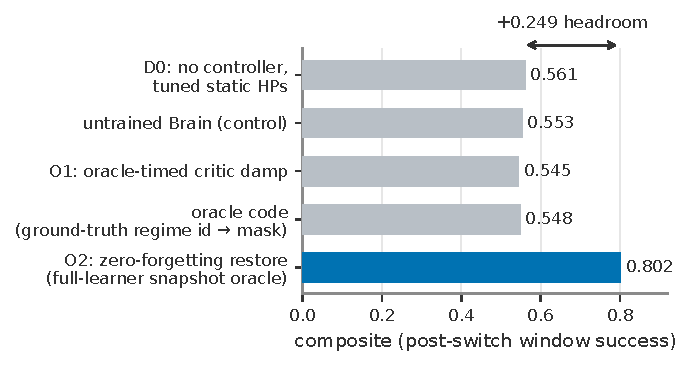
\includegraphics[width=0.78\linewidth]{figures/fig1_ladder.pdf}
  \caption{\textbf{The control ladder} (box protocol, $n{=}8$ runs per rung).
  Every controller rung --- none, untrained, oracle-assisted --- lands within
  $\pm 0.008$ of the untrained-Brain control, while the zero-forgetting
  restore oracle (O2) gains $+0.249$. The bottleneck is knowledge
  restoration, not learning dynamics.}
  \label{fig:ladder}
\end{figure}

\begin{table}[t]
  \centering
  \caption{\textbf{Control ladder} on the frozen benchmark (box protocol;
  $n{=}8$ per rung; control CI from $n{=}32$). \composite{} integrates
  post-switch recovery; \hit80{} is threshold-recovery reliability.}
  \label{tab:ladder}
  \small
  \begin{tabular}{lccl}
    \toprule
    Rung & \composite{} & \hit80{} & Reading \\
    \midrule
    D0 --- no controller, tuned static HPs & 0.561 & 0.786 & static baseline is strong \\
    Control --- untrained Brain (noise actions) & 0.553\,{\scriptsize[0.548, 0.559]} & 0.829 & jitter buys reliability, not mean \\
    O1 --- oracle-timed critic-LR damping & 0.545 & 0.806 & \emph{hurts}: whiplash is functional \\
    Oracle code --- true regime id $\to$ mask & 0.548 & 0.826 & gating pathway inert \\
    O2 --- zero-forgetting restore (oracle) & \textbf{0.802}\,{\scriptsize(sd 0.009)} & 0.873 & $+0.249$ headroom \\
    \bottomrule
  \end{tabular}
\end{table}

Each rung replaces exactly one ingredient of the full system
(Table~\ref{tab:ladder}, Figure~\ref{fig:ladder}); all rungs run the identical
benchmark, protocol, and scorer.

\textbf{D0 (no controller).} The Brain is severed and every lever is pinned to
the midpoint of its range --- empirically the operating point trained Brains
settle at. D0 scores $0.561$ \composite{} and reaches the 80\% threshold on
79\% of switches. This matters twice. First, it corrects a weak-baseline
artifact: an earlier report on this system claimed a static learner ``never
reaches 80\%'' post-switch (scoring it 0.464) and credited the difference to
the controller; the tuned static baseline in fact sits \emph{above} the
untrained-controller control. Second, comparing D0 to the control isolates
what an untrained controller contributes: its action jitter \emph{costs}
composite but buys $+4$ points of \hit80{} --- exploration noise as an
accidental reliability mechanism.

\textbf{O1 (oracle-timed critic damping).} A hypothesized pathology was
post-switch critic ``whiplash'' (large value-error transients driving biased
advantage estimates). O1 damps the critic learning rate for a window after
each \emph{ground-truth} switch --- perfect timing, upper-bounding any learned
damping schedule. It mildly hurts both metrics ($0.545$/$0.806$). The critic's
violent post-switch re-fit is the mechanism doing its job, not a failure mode
--- a caution against ``stabilizing'' interventions that treat transients as
pathologies (cf.\ pathological value dynamics studied
in~\citep{kumar2021implicit,lyle2022capacity}).

\textbf{Oracle code (pathway test).} The 8-d context code is replaced by
ground-truth regime identity --- the information the code could at best learn
to convey. Result: $0.548$/$0.826$, indistinguishable from control. The
modulation \emph{pathway} is inert even with perfect information: a
suppressive mask over one shared feature vector cannot store two policies, it
can only choose what to compute with the single set of weights it has. This
retroactively explains the nulls of three screening families
(\S\ref{sec:audit}) and gives our instrument's version of the XdG
lesson~\citep{masse2018xdg}: gating without memory has a low ceiling.

\textbf{O2 (zero-forgetting ceiling).} At each ground-truth switch, the
learner's full state --- policy network, world model, and both optimizer
states --- is snapshotted under the outgoing regime and the stored state for
the incoming regime is restored. O2 scores $\mathbf{0.802}$ \composite{}
(sd $0.009$): $+0.249$ over control, with low variance. Two readings die
here: ``the benchmark has no headroom'' and ``the metric cannot see
improvements.'' What remains is an attribution question we return to in
\S\ref{sec:limitations}: the snapshot restores policy memory, world-model
memory, and optimizer curvature together, so O2 bounds \emph{knowledge
restoration in aggregate}, and decomposing which component carries the
$+0.249$ is the first experiment of the follow-up program.

\textbf{Plasticity probe.} Alongside the ladder we measured the dormant-unit
fraction~\citep{sokar2023dormant} of the inner learner's actor/critic heads
over the run. It \emph{falls} from $0.9$ (fresh initialization) to $0.35$ and
never re-accumulates across switches. Plasticity loss --- the failure mode
targeted by reset-style
interventions~\citep{dohare2024plasticity,nikishin2022primacy} --- is absent
at this horizon and scope, consistent with that literature's own observation
that the effect needs much longer non-stationary exposure~\citep{abbas2023plasticity,nikishin2023injection}.

\section{Does Training the Controller Help?}
\label{sec:replication}

The ladder bounds what meta-control could do; this section measures what
trained meta-control \emph{does}, under the tightest contrast we could build,
and then replicates it across the axis that single-system studies leave
unvaried: the controller's own training seed.

\subsection{Single-variable matched contrast}
\label{sec:contrast}
The contrast compares a \emph{trained} Brain checkpoint against the
\emph{same architecture at random initialization}, holding everything else
fixed: identical benchmark, schedule, inner learner, and evaluation protocol
(16 inner environments, controller acting every update); the controller's
weights are the only variable. Both arms are evaluated frozen (no outer
learning during evaluation), across disjoint evaluation seeds. For the
original controller --- a single Brain trained in March~2026 (130 episodes,
seed~0) --- the contrast gives trained $0.5577$ (sd $0.051$) vs.\ init
$0.5285$ (sd $0.022$): $\Delta = +0.0292$, Welch $t\approx2.97$, $p<0.01$ at
$n{=}32$ evaluation seeds per arm. Three properties distinguish this from the
mirages of \S\ref{sec:mirages}: the estimate \emph{converged} with sample size
($+0.046 \to +0.028 \to +0.029$ at $n{=}8/16/32$); the effect is dose-ordered
(init $<$ ep91 $<$ ep130 across checkpoints of the same run); and \hit80{} is
identical between arms (0.982 both) --- the gain is purely mean recovery, with
no reliability claim.

\subsection{Replication across training seeds}
A single trained controller supports only the existential claim ``there
exists a Brain that helps'' --- and outer-loop meta-RL training is exactly
where high seed variance should be expected~\citep{henderson2018matters,colas2018seeds}.
We therefore pre-registered (predictions, selection rule, gates, and failure
reading committed before any new controller existed) a replication across
four fresh Brains, seeds 1--4, trained at the March configuration. Design
safeguards: each Brain's \emph{own} initialization is saved at episode~0 and
serves as its matched control arm; checkpoint selection uses the documented
training-reward rule (\S\ref{sec:instrument}), applied before evaluation ---
it picked the final checkpoint (ep130) for all four Brains; evaluation
proceeds up an $n{=}8 \to n{=}16$ ladder with the convergence-vs-decay
criterion applied at each rung. The pre-registered success gate (P-R1a) was:
pooled $\Delta > 0$ at $p<0.01$ \emph{and} at least 3 of 4 Brains
directionally positive.

\begin{figure}[t]
  \centering
  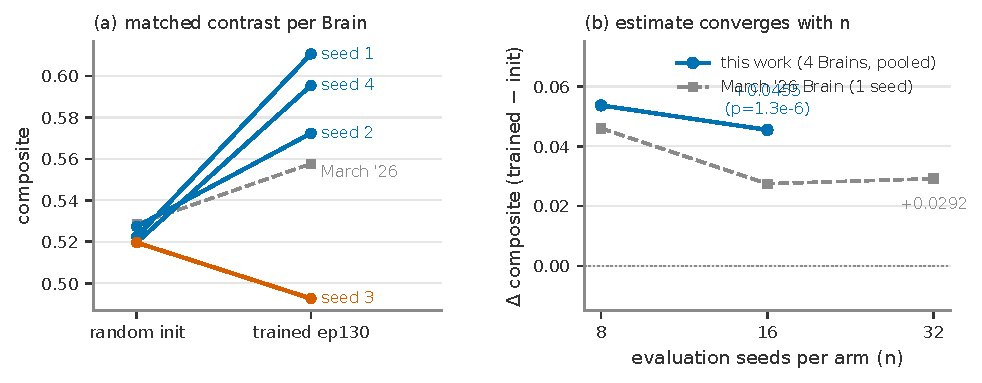
\includegraphics[width=\linewidth]{figures/fig2_replication.pdf}
  \caption{\textbf{The trained-controller effect replicates across training
  seeds.} (a) Matched contrast per Brain at $n{=}16$ evaluation seeds per arm
  (March campaign: $n{=}32$, dashed): three of four fresh Brains improve on
  their own initialization; seed~3 is a genuinely negative training draw.
  (b) The pooled estimate \emph{converges} as evaluation samples grow --- the
  signature that separated this effect from three small-sample mirages
  (\S\ref{sec:mirages}), each of which decayed toward zero under the same
  treatment.}
  \label{fig:replication}
\end{figure}

\begin{table}[t]
  \centering
  \caption{\textbf{Multi-seed replication} (evaluation protocol; $n{=}16$
  evaluation seeds per arm per Brain; Welch's $t$). Each Brain is contrasted
  with its own frozen episode-0 initialization. March campaign shown for
  comparison ($n{=}32$/arm).}
  \label{tab:replication}
  \small
  \begin{tabular}{lcccccc}
    \toprule
    Brain & init & trained & $\Delta$ & $p$ & \hit80{} (tr/init) \\
    \midrule
    seed 1 & 0.5225 & 0.6107 & $+0.0881$ & $2.1\times10^{-5}$ & 0.982 / 0.964 \\
    seed 2 & 0.5274 & 0.5724 & $+0.0450$ & $1.5\times10^{-3}$ & 0.973 / 0.964 \\
    seed 3 & 0.5196 & 0.4926 & $-0.0270$ & $0.046$            & 0.929 / 0.955 \\
    seed 4 & 0.5197 & 0.5955 & $+0.0758$ & $3.9\times10^{-6}$ & 0.991 / 0.964 \\
    \midrule
    \textbf{pooled (4 seeds)} & \textbf{0.5223} & \textbf{0.5678} & $\mathbf{+0.0455}$ & $\mathbf{1.3\times10^{-6}}$ & 0.969 / 0.962 \\
    March '26 (1 seed, $n{=}32$) & 0.5285 & 0.5577 & $+0.0292$ & $<0.01$ & 0.982 / 0.982 \\
    \bottomrule
  \end{tabular}
\end{table}

\textbf{Results} (Table~\ref{tab:replication}, Figure~\ref{fig:replication}).
The gate passed. Pooled over the four fresh Brains: trained $0.5678$ (sd
$0.066$) vs.\ init $0.5223$ (sd $0.020$), $\Delta = +0.0455$, $t=5.27$,
$p=1.3\times10^{-6}$ at $n{=}16$/arm, converged from $+0.0537$ at $n{=}8$.
Three of four Brains are individually positive; seed 3 finished trained yet
scores \emph{below} its own initialization --- with only four training seeds
we report the spread verbatim rather than averaging it away (a cross-seed
$t$-test at $\mathrm{df}{=}3$ would be theater; the claim rests on the pooled
evaluation contrast plus per-seed directionality, as pre-registered). Init
arms are tightly consistent across all five Brains ($0.520$--$0.529$),
matching the ladder's untrained rungs. The pooled effect \emph{exceeds} the
March estimate --- the original controller was a below-median draw, not a
lucky one. Under the pre-registered decision rule, the claim upgrades from
existential to distributional: \textbf{Brains trained this way improve
post-switch recovery, across training draws}, at $\sim$9\% relative composite
--- and $\sim$18\% of the O2 ceiling.

\section{Three Mirages and a Criterion}
\label{sec:mirages}

The positive result above is the survivor of a screening program in which
three other effects looked at least as good and died. We document them
because the discipline that killed them is, we believe, as reusable as the
result --- an in-vivo confirmation of published warnings about small-$n$ RL
comparisons~\citep{henderson2018matters,colas2018seeds,agarwal2021precipice}
from inside a single research program.

\textbf{The mirages.} (i) A critic-side use of the context code showed a
reliability gain at $n{=}3$ and survived a mechanical holdout check; it died
at $n{\geq}8$. (ii) An auxiliary code-prediction loss at increased coefficient
showed the same signature at $n{=}3$; died at $n{\geq}8$. (iii) A
dormant-neuron reset intervention (in the spirit
of~\citep{sokar2023dormant,nikishin2022primacy}) passed at $n{=}6$, then died
at $n{=}10$ --- and its registered mechanism probe showed the quantity it
resets never accumulates in the first place (\S\ref{sec:ladder}). All three
were plausible, literature-backed, and initially significant.

\textbf{The criterion.} Track the effect estimate as evaluation samples grow.
Sampling artifacts \emph{decay} toward zero (each looked strongest at its
smallest $n$); real effects \emph{converge} to a stable value. The March
contrast converged ($+0.046 \to +0.028 \to +0.029$); the replication converged
($+0.054 \to +0.046$); all three mirages decayed. The criterion is a
complement to, not a substitute for, adequate $n$ and proper
CIs~\citep{agarwal2021precipice}: its value is as a pre-registered
\emph{stopping rule} for scaling up --- and as a cheap early kill for effects
that will not survive it. Where affordable we also attach mechanism probes
(the dormant-fraction probe killed mirage~(iii) independently of its score)
and dose orderings (\S\ref{sec:contrast}).

\textbf{The protocol confound.} Evaluation and screening configurations that
differ in seemingly innocuous ways are not comparable. Measured at identical
hyperparameters, moving from our screening protocol to our evaluation
protocol shifts \composite{} by $-0.045$ and \hit80{} by $+0.18$ --- the
16-environment evaluation smooths the success trace enough to inflate
threshold-crossing statistics massively. An early ``reliability gradient''
claim in this project (a trained Brain re-attaining threshold on 64/64
switches) dissolved on protocol-matched controls: an \emph{untrained} Brain
at the evaluation protocol already re-attains on 96.4\% of switches, putting
64/64 at $p\approx0.10$. Every claim in this paper is within-protocol;
every cross-protocol number we report is labeled as such.

\textbf{The instrument audit} (\S\ref{sec:audit}) belongs to the same family:
before asking whether a mechanism improves a learned controller, verify the
controller in the loop is trained. We suspect this failure mode ---
structurally invisible from inside the pipeline, since every cell is affected
equally --- generalizes to other automated evaluation systems.

\section{Discussion}
\label{sec:discussion}

\paragraph{What the ladder buys.}
A single uncontrolled comparison --- trained system vs.\ ad-hoc baseline ---
would have reported $+0.10$ or more on this instrument and attributed it to
neuromodulation (an earlier report on this system did exactly that). The
ladder decomposes that number into: a weak-baseline artifact (D0), a
reliability effect of action noise (control vs.\ D0), an inert gating pathway
(oracle code), a functional transient misread as pathology (O1), a real but
small trained-controller effect ($+0.046$, \S\ref{sec:replication}), and a
large untouched restoration headroom ($+0.249$, O2). We think this
decomposition, not any single rung, is the paper's main methodological
export.

\paragraph{Why is trained meta-control small here when it is large elsewhere?}
The stationary successes~\citep{xu2018metagradient,zahavy2020stac} tune the
learner \emph{toward a fixed optimum}; under regime cycling, the knowledge
the learner needs was already acquired and then overwritten --- and no
learning-rate or exploration schedule can un-overwrite it. The XdG
combination lesson~\citep{masse2018xdg}, the memory-restoration reading of
reset methods~\citep{klein2024plasticitysurvey}, and our O2 rung all point the
same way: dynamics levers modulate the \emph{speed} of relearning; memory
levers change \emph{whether relearning is necessary}. On our instrument the
speed channel is worth $\sim$0.05 and the necessity channel $\sim$0.25.

\paragraph{The next instrument: learned restoration.}
O2 is an oracle in two places --- \emph{when} to restore (ground-truth switch
times) and \emph{what} to restore (ground-truth regime identity). Both are
learnable targets: the Brain's own observation already carries switch-timing
signals (surprise spikes), and selection among $K{=}2$ snapshots is a single
bit. The follow-up program, pre-registered in outline, therefore replaces the
inert code dimensions of the action space with memory-facing levers ---
snapshot commit, restore trigger, slot selection --- and asks what fraction
of the $+0.249$ a \emph{learned} trigger recovers, with the decomposition of
the O2 snapshot (policy vs.\ world model vs.\ optimizer state) as the routing
experiment. The four replicated Brains of \S\ref{sec:replication} are the
baseline arm of that comparison. Buffer-selection results
suggest the selection half is where the difficulty
concentrates~\citep{isele2018selectivereplay,kessler2023continualdreamer};
our regime pair, differing only in reward, makes the world-model component of
the snapshot nearly free to bank, which the decomposition can exploit.

\paragraph{For the neuromodulation literature.}
Our negative pathway result does not contradict demonstrations that gating
channels can be powerful~\citep{beaulieu2020anml,serra2018hat,miconi2019backpropamine}
--- in those systems the gate is trained through, per-input, and effectively
\emph{is} a memory (a mask that partitions capacity). It does say that a
low-dimensional, outer-emitted, multiplicative code over a shared
representation --- the form neuromodulation often takes in two-level RL
proposals --- has no mechanism to store anything, and ground-truth information
through it does nothing. Proposals of this form should be accompanied by an
oracle-information rung; ours took one GPU-day and settled the question.

\section{Limitations}
\label{sec:limitations}

\textbf{One instrument.} All results are on one small, fully controlled
benchmark family (MiniGrid goal regimes, 2 regimes, $8{\times}8$). The regime
pair shares dynamics and differs only in reward; restoration may be harder
when dynamics shift too. Cyclic two-regime protocols structurally favor
restoration~\citep{powers2022cora}, and forward transfer --- argued by
\citet{wolczyk2021continualworld} to be the harder frontier --- is outside our
metric's scope. The instrument was chosen to make the control ladder
affordable; porting the ladder to richer benchmarks is future work, not a
claim we make.

\textbf{O2 is an aggregate bound.} The snapshot restores policy, world model,
and optimizer state together; we have not yet attributed the $+0.249$ among
them. It bounds knowledge restoration in aggregate and is not evidence for
any particular memory mechanism --- notably, naive replay can interfere in
exactly this regime type~\citep{kessler2023continualdreamer}.

\textbf{Controller scope.} The Brain is a small MLP with a fixed 15-d
interface and no recurrence; its observation carries no regime identity. A
controller with memory over its own history, or richer observations, might
capture more of the ceiling --- that is part of the follow-up program, not a
tested claim.

\textbf{Statistical scope.} Four training seeds bound what we can say about
the training-draw distribution (one of four was negative); the pooled claim
is about evaluation-seed uncertainty given these Brains, plus directionality.
The dormant-fraction probe covers the actor/critic heads at this horizon;
encoder-side dormancy was not separately measured. \composite{} is one facet
of recovery; we report \hit80{} alongside but make no reliability claims.

\section*{Reproducibility statement}
The benchmark, scorer, and evaluation adapters were frozen before the
experiments reported here; the replication's predictions, checkpoint-selection
rule, success gate, and failure reading were committed to version control
before any of the four Brains existed. All headline numbers were re-scored
from raw evaluation logs on a second machine with the same frozen scorer.
Training seeds fully determine controller initialization (verified
reproducible and pairwise distinct); every evaluation cell's seed is recorded.
Code, configurations, evaluation logs, and the pre-registration history will
be released \todo{anonymized repository link at submission}.

\bibliographystyle{plainnat}
\bibliography{references}

\appendix

\section{Instrument configuration}
\label{app:config}

\begin{table}[h]
  \centering
  \caption{Controller lever bounds (actions mapped linearly from $[-1,1]$;
  D0 pins each lever to its midpoint).}
  \small
  \begin{tabular}{lcc}
    \toprule
    Lever & min & max \\
    \midrule
    inner learning rate & $10^{-4}$ & $3\times10^{-3}$ \\
    entropy coefficient & $10^{-3}$ & $0.1$ \\
    intrinsic coefficient & $10^{-3}$ & $0.5$ \\
    imagined-rollout horizon & $1$ & $30$ \\
    replay ratio & $0$ & $0.5$ \\
    replay prioritization & $0$ & $1.0$ \\
    anchoring weight & $0$ & $0.5$ \\
    \bottomrule
  \end{tabular}
\end{table}

\noindent Inner learner: 16 environments $\times$ 128-step rollouts, 800k
steps per run, 100k steps per regime (7 switches), episodic memory capacity
100k, world-model learning rate $10^{-4}$, imagination horizon initialized at
10. Outer training: 8 parallel inner runs, 130 episodes, Adam ($10^{-4}$),
recovery reward ($\alpha{=}0.1$, $\beta{=}0.5$), controller acting every inner
update. Evaluation protocol: 16 inner environments, controller frozen,
disjoint evaluation seeds per arm. Scoring: post-switch window = 500-step
buffer, then 50\% of a regime; \hit80{} sustain = 3 consecutive logged points.

\end{document}
